\title{Solomonoff Library Specification and Technical Documentation}
\author{Aleksander Mendoza-Drosik}

\documentclass[12pt]{article}
\usepackage{tikz}
\usepackage[utf8]{inputenc}
\usepackage[T1]{fontenc}
\usepackage{lmodern}
\usepackage{amsfonts}
\usepackage{mathrsfs}
\usepackage{centernot}
\usepackage{listings}
\usepackage{mathtools}
\usepackage{xcolor}
\usepackage{url}
\usepackage{hyperref}
\usepackage{amsthm}
\usepackage{amsmath}
\usepackage{amssymb}
\usepackage{syntax}
\newtheorem{definition}{Definition}
\newtheorem{theorem}{Theorem}[section]
\newtheorem{corollary}{Corollary}[theorem]
\newtheorem{lemma}[theorem]{Lemma}
\renewcommand{\labelenumii}{\theenumii}
\renewcommand{\theenumii}{\theenumi.\arabic{enumii}.}
\DeclareMathSymbol{:}{\mathord}{operators}{"3A}

\begin{document}
\maketitle
\lstset{
	basicstyle=\ttfamily,
	mathescape
}

 \section{Introduction}

Solomonoff is a compiler backend for assembling  transducers. 
It employs a range of extensions such as lexicographic weights, symbolic transitions, reflection outputs and more. 

The automata are represented using singly-linked graph $G$. Each vertex $N$ stores some assigned state value $V$ and keeps track of its own outgoing edges. Each edge stores the pointer to target vertex and some associated value $E$, often used for representing automaton's transition. The advantage of such data structure is that adding and removing edges is a constant operation that does not depend on size of graph. The downside is that such graphs do not have a "well defined" set of vertices. Any object $N$ can be considered as vertex of $G$ that just happens to be disconnected from rest of the graph. One might formally think that there exists one and only graph $G$ that consists of many connected components. Each such connected component is defined by a selected vertex $N$ and all other vertices  reachable from it. 

The graph becomes an automaton when in addition to vertices and edges we also keep track of initial and final states. Having a set of initial vertices, the automaton consist of the union of all the reachable connected  components. Solomonoff makes extensive use of Glushkov's construction. The automata produced as a result have the very specific property that the unique initial state cannot have any incoming transitions. The optimal data structure for representing such automata is the singly-linked graph together with set of "initial" and "final" edges.
The initial (or final) edgs can be thought of as "partial"  edges  that only have target (source) vertex but the source (target) vertex is not known yet. In such a setting, the unique initial state is implied. It only exists "logically" as the source vertex of all partial initial edges but is not "physically" specified in the data structure itself. In addition to initial and final transitions, Glushkov's construction also requires keeping track of whether or not the empty word is accepted. To represent this we use epsilon edge that belongs to graph but whose neither source nor target vertex is known. Hence epsilon transition could be visualised as a "partial" edge that freely floats next to the graph structure but is not attached anywhere. 

This data structure has intricate connection to subsequential transducers, which are defined as having state output in addition to transition output. When subsequential transducer accepts its total output is obtained by concatenating outputs of all consecutive transitions and then appending the state output at the very end. We could imagine that the "final" edges exactly correspond to state output. It makes sense, because as we will soon see, Glushkov's construction only requires one unique final edge per state. States that are not accepting can be modelled as particular case of accepting subsequential states, whose output is the null element $\emptyset$ (note that in Kleene algebra, the empty set $\emptyset$ works as multiplicative zero such that $\emptyset \cdot a = a \cdot \emptyset = \emptyset$ for any string $a$, hence such state output annihilates all the transition outputs). Such a setting is especially convenient in Java (the language, which Solomonoff was implemented in), because $\emptyset$ can be literally represented using \texttt{null} and when we perform lookup of final edge in \texttt{HashMap} for some particular vertex, we get \texttt{null} whenever the vertex did not belong to the map. 
Interestingly, the epsilon edge "logically" correspond to the output of initial state. Every detail in our implementation perfectly fits together.

Note that at no point in the above definition, we made any mentions of the alphabet. The edges $E$ are meant to hide the alphabet behind a layer of abstraction. We are allowed to iterate all the outgoing transitions $E$ of any state $N$ and we can lookup the target state $N$ for any source state $N$ and outgoing edge $E$, but we are not allowed to ask, which edges $E$ transition over specific input symbol $\Sigma$. That is because, the edges are in fact symbolic. Every $E$ spans a range of symbols and there is no 1-to-1 correspondence between edges and symbols. In theory, each edge $E$ might represent an arbitrary predicate. It would be relatively easy to assemble transducers that work over real or complex numbers, trees, matrices or any other data structures. Solomonoff implements the approach that input alphabet $\Sigma$ is represented using 64-bit integers and each transition could span arbitrary range of the form $c_1 < \sigma \le c_2$ for any constants $c_1$ and $c_2$. The inequality $<$ is on the left side for a good reason. Solomonoff assumes the existence of special minimal symbol $\bot$ such that $\bot \notin \Sigma$ and $\bot < \sigma$ for any symbol $\sigma$. The $\bot$ has a special meaning and is later used for reflections. It's also easy to cover entire the $\Sigma$ only by specifying  consecutive breakpoints. Given a sequence of edges  $E_0,E_1,E_2,...E_n$ we can always find all the constants $c_1<c_2<c_3<...<c_m$ such that every $c_i$ appears (as upper bound $c_k<\sigma\le c_i$  or as  lower bound $c_i<\sigma\le c_k$) in some (one or more) $E_j$. Then we can build a very efficient lookup table $T$ that to every $c_i$ associates set of edges such that $E_h \in T(c_i)$ whenever $E_h$ spans some range $c_u < c_i \le c_v $ containing $c_i$. Then in order to lookup $T(\sigma)$, we perform binary search on $c_1<c_2<c_3<...<c_m$ and find the least upper bound $\sigma \le c_i$. This way, Solomonoff is able to perform quick lookups even when alphabets span millions of symbols.

The lookup table is not built during Glushkov's construction. Instead the compilation is split into two phases. First the singly-linked graph $G$ is built. This data structure is mutable and can perform edge insertions/deletions efficiently, but lookup of edge by symbol requires linear search. In the second phase, $G$ is compiled to array of states. In order to do that, all reachable vertices of $G$ scanned and assigned some unique. Then and array is built, such that element at a given index contains the lookup table of all transitions outgoing from the corresponding vertex. Such optimised data structure is immutable but can be executed efficiently.  



 \section{Code conventions}

Solomonoff is written in Java using the "typeclass pattern". Almost everything is an interface. Each of the interfaces corresponds to some formal mathematical definition and stores a handful of axioms (each axiom is a method). Non-axiom methods are canonically represented as pure static functions. 
For example consider set of finite sequences $\Omega_X$ of elements from set $X$. A string $\sigma_1\sigma_2\sigma_1$ over alphabet $\Sigma=\{\sigma_1,\sigma_2\}$ might be represented as a sequence $\langle \sigma_1,\sigma_2,\sigma_1\rangle$ of $\Omega_\Sigma$. An axiomatization of finite sequences might be a (dependent) pair $(n, f)$ of some number $n$ and function $f$ that to every integer between $0$ and $n$ assigns some element of $X$. Formally written as $(n, f) : \mathbb{N} \times (0...n \rightarrow X)$. Then in Java we could represent it as class
\begin{lstlisting}[language=java, escapeinside={(*}{*)}]
class (*$\Omega$*)<X>{
    int n();
    X f(int i); //requires 0<=i<n
}
\end{lstlisting}
Then a function that operates on $\Omega_X$, like concatenation for instance, would have to be represented using a pure static method.
\begin{lstlisting}[language=java, escapeinside={(*}{*)}]
static <X> (*$\Omega$*)<X> concat((*$\Omega$*)<X> left, (*$\Omega$*)<X> right){...}
\end{lstlisting}
Sometimes, different implementations of $\Omega_X$ might use different underlying data structures, which in turn allow for more efficient implementations of certain functions. For example the generic implementation of \texttt{concat} might create a new instance with a new backing array and copy the elements of the two previous sequences. However, if we know that the exact implementation uses linked lists, a much more efficient procedure could work in constant time.  For this reason Solomonoff sometimes defines the non-axiomatic methods directly as part of interface, not because they are necessary, but because can be implemented more efficiently. The programmer should still be aware of the underlying formal specification. 

Our Java code also strictly follows the specification of linear types. Even though Java compiler does not have any support for borrowing, ownership and lifetimes, that does not mean the code cannot be properly annotated in such a manner. For example consider the above definition of \texttt{concat}. It might produce a new instance for each call, but a more efficient implementation would mutate one of the arguments. The only problem is that mutations might leads to bugs and data races when not used properly. To avoid that, we explicitly specify (in the comments), which function arguments are linear.
For instance, if we specified that \texttt{left} argument is "consumed", then we should ever use it after calling \texttt{concat}. Suppose that $\Omega_X$ is implemented using linked lists and the right argument is appended to the left one. We could write something like this to concatenate \texttt{a + b1 + b2}
\begin{lstlisting}[language=java, escapeinside={(*}{*)}]
concat(a,b1);
concat(a,b2);
\end{lstlisting}
but this solution might break as soon as the implementation is changed. The canonical way of writing code with linear types would be instead
\begin{lstlisting}[language=java, escapeinside={(*}{*)}]
a2 = concat(a,b1);
//a is consumed and should never be touched again!
a3 = concat(a2,b2);
//a2 is consumed and should never be touched again!
\end{lstlisting}
 Programmer must also keep in mind that in order to invoke \texttt{concat(left,right)} we must also make sure that we own the \texttt{left} argument. If a reference to this variable was simultaneously used in some other place and we consumed it here, that other place would have no way of knowing that \texttt{left} is no longer valid. Therefore attention must be paid whenever we copy references from one place to the other (which is commonly known as "borrowing"). 
 
 Every function that mutates its arguments, can also be represented as linear function without mutations. For instance 
  \begin{lstlisting}[language=java, escapeinside={(*}{*)}]
static <X> void concat((*$\Omega$*)<X> left, (*$\Omega$*)<X> right)
 \end{lstlisting}
 is the mutating version of 
 \begin{lstlisting}[language=java, escapeinside={(*}{*)}]
 /**consumes left*/
static <X> (*$\Omega$*)<X> concat((*$\Omega$*)<X> left, (*$\Omega$*)<X> right)
 \end{lstlisting}
 In object-oriented languages we have one more possible approach
 \begin{lstlisting}[language=java, escapeinside={(*}{*)}]
void concat((*$\Omega$*)<X> right)
 \end{lstlisting}
 where \texttt{this} instance is implied to be linear (\texttt{this=left}).
 
In Solomonoff, the convention is to use the second approach for static functions, but third approach whenever the method is part of an interface, although there are some exceptions. In particular, note that the static functions require all generic arguments to be mentioned explicitly. When there are too many of them, it becomes more convenient and readable to turn static methods into interface methods and let all the generics be declared only once globally as the interface generics. Instead of
 \begin{lstlisting}[language=java, escapeinside={(*}{*)}]
static <X1,X2,X3,Y> Y f1(X1 x1, X2 x2, X3 x3){...}
static <X1,X2,X3,Y> Y f2(X1 x1, X2 x2, X3 x3){...}
\end{lstlisting}
we obtain more concise notation
 \begin{lstlisting}[language=java, escapeinside={(*}{*)}]
interface ShareGenerics<X1,X2,X3,Y>
    default Y f1(X1 x1, X2 x2, X3 x3){...}
    default Y f2(X1 x1, X2 x2, X3 x3){...}
}
\end{lstlisting}
This approach should be considered merely as syntactic sugar. Those functions are usually not meant to be extended in any way. Most of the methods in Solomonoff are pure and do not have any state. Even the seemingly impure functions become pure when linear logic is taken into account. 


 
 \section{Singly linked graphs}
 
We formally define singly-linked graph $G$ over set of vertices $N$ and edges $E$ as product $G= N \times E \times N$, where $(n_1,e,n_2)\in G$ should be understood as edge outgoing from $n_1$ and incoming to $n_2$ with label $e$. We also define mapping $v : N \rightarrow V$ from vertices to states $V$.
Java implementation of $G$ together with $v$ is represented as the class \texttt{SinglyLinkedGraph<V, E, N>}. The axioms are

 \begin{lstlisting}[language=java]
V getState(N vertex)
void setState(N vertex, V v)
Map<E, N> outgoing(N from)
N create(V state)
void add(N from, E edge, N to)
boolean remove(N from, E edge, N to)
\end{lstlisting}


There are also two very important implicit axioms for $N$ and $E$. The \texttt{n1.equals(n2)} is true if and only if the vertex instances are the same \texttt{n1==n2}. Similarly for edges \texttt{e1.equals(e2)}. Hence the map \texttt{Map<E, N>} implies that the target is uniquely determined by the edge. Hence $G$ is actually a function $G= N \times E \rightarrow N$.

For convenience we also define the mapping 
 \begin{lstlisting}[language=java]
Object getColor(N vertex)
void setColor(N vertex, Object color)
\end{lstlisting}
 which to every vertex assigns some "color". Here color is to be understood as auxiliary piece of information that can be stored in each vertex. It is useful whenever some procedure requires to perform additional bookkeeping of temporary values. For example, the \texttt{pseudoMinimize} procedure uses "color" for temporarily storing edges incoming to every vertex. 
 
Let $P$ be some set of partial outgoing edges. Then automaton is obtained by combining $G$ together with initial edges $E \rightarrow N$, final edges $N\rightarrow P$ and one epsilon edge $p_\epsilon \in P \cup \{\emptyset\}$ which might be null. Java implements this as \texttt{IntermediateGraph<V, E, P, N>}. 
It's axioms are
 
 \begin{lstlisting}[language=java]
P getEpsilon()
void setEpsilon(P epsilon)
Map<E, N> allInitialEdges()
Map<N, P> allFinalEdges()
 \end{lstlisting}


 \section{Transducers}
 
 The heart of Solomonoff lies in the interface \\
 \texttt{Specification<V, E, P, In, Out, W, N, G>}. \\
 Let $\Sigma$ be the input alphabet ($\Sigma \cup \{\bot\}$\texttt{=In} in Java), $O$ be the set of output values ($O\cup\{\emptyset\}$\texttt{=Out} in Java) and $W$ the set of transition weights. The $O$ and $W$ are required to be monoids. The axioms are
  
 \begin{lstlisting}[language=java]
Out multiplyOutputs(Out lhs, Out rhs)
W multiplyWeights(W lhs, W rhs)
W weightNeutralElement()
Out outputNeutralElement()
 \end{lstlisting}
 

 
 Assume a total order $\le$ on $\Sigma$. A range $R_\texttt{In}$ over \texttt{In} is a pair $(\sigma_1,\sigma_2]$. An element $\sigma$ belongs to range $(\sigma_1,\sigma_2]$ if and only if $\sigma_1<\sigma\le\sigma_2$. The element $\sigma_1$ is the (exclusive) lower bound and $\sigma_2$ is the (inclusive) upper bound). Let there be a mapping $\pi$ from edges $E$ to ranges $R_\texttt{In}$. Because a range is a pair of elements, it's often more convenient to represent $\pi$ as two separate mapping $\pi_1$ and $\pi_2$ that map each edge to the lower/upper bound respectively. The axioms are
   
 \begin{lstlisting}[language=java]
In fromExclusive(E edge)
In toInclusive(E edge)
In successor(In predecessor)
In minimal() 
In maximal()
int compare(In point1, In point2)
 \end{lstlisting}
 It is assumed that minimal symbol of \texttt{In} is the element $\bot$,  which does not belong to $\Sigma$.
 
 The monoids of $O$ and $W$ can be used to form a direct product $O\times W$. There must exist a homomorphism $\phi$ from   partial edges $P$ to $O\times W$. If $\phi(p)=(o_1,w_1)$ then $\phi(o_2 p)=o_2\phi(p)=o_2(o_1,w_1)=(o_2o_1,w_1)$  and $\phi(w_2 p)=w_2\phi(p)=w_2(o_1,w_1)=(o_1,w_2w_1)$, hence $O$ and $W$ act on $P$. The partial edges should themselves form a monoid and $O\times W$ should be a quotient of $P$, such that $\phi(o_1,w_1)\phi(o_2,w_2)=\phi(o_1o_2,w_1w_2)$. This homomorphism is implicitly assumed to exist, but is not explicitly specified in Java code. Instead much more important is the embedding $\phi^{-1}:O\times W\rightarrow P$. The exact axiomatization is as follows
 
 \begin{lstlisting}[language=java]
P multiplyPartialEdges(P edge, P edge2)
P createPartialEdge(Out out, W weight)
 \end{lstlisting}
 
Furthermore, despite $E$ not being a monoid by itself, $P$ is in a sense a "quotient set" of $E$. Similarly to how $O\times W$ can act on $P$, the set $P$ can both act on and be embedded in $E$. Indeed $E$ can be treated like $E=P\times R_\Sigma$ and it should satisfy $(op,r)=o(p,r)$ and $(po,r)=(p,r)o$ where $p\in P, o\in O,r\in R_\texttt{In}, (p,r)\in E$.  The axioms are
 
 \begin{lstlisting}[language=java]
E leftAction(P edge, E edge2)
E rightAction(E edge, P edge2)
 \end{lstlisting}
 
 All those axioms together give us full specification of $\Sigma$, $O$ and $W$ along with ways to manipulate transitions.  The last thing we need is a graph constructor 
 \begin{lstlisting}[language=java]
G createEmptyGraph()
 \end{lstlisting}
 
 
\section{Glushkov's construction}
  
While most compilers built abstract syntax tree, Solomonoff skips this stage and produces automata instantaneously as parsing progresses. This process is performed in \texttt{ParserListener<Pipeline, Var, V, E, P, A, O, W, N, G>}. Our language of regular expressions has been specifically designed to work with functional transducers, which are non-deterministic but guarantee at most one output for each input. Most other transducer libraries implement syntax that looks as follows:
\begin{grammar}
	
	<regex> ::= <regex>  <regex> // concatenation
	\alt <regex> `|' <regex> //union
	\alt <regex> `*'              //Kleene closure
	\alt <regex> `:' <regex> //input-output product
	\alt <atomic> 
	
\end{grammar}
Solomonoff goes with a very different approach
\begin{grammar}
	
	<regex> ::= <regex>  <regex> // concatenation
	\alt <regex> `|' <regex> //union
	\alt <regex> `*'              //Kleene closure
	\alt `:' <atomic> //output string
	\alt <atomic> //input string
	
\end{grammar}
This makes a significant difference, because in the first approach regular expression like $(a:b):c$ evaluates to $a:c$. The $lhs:rhs$ works as cross product between inputs of left-hand-side with inputs of right-hand-side. Then every single input accepted by $lhs$ produces all of the accepted inputs of $rhs$ as its new outputs and the original outputs of $lhs$ are lost. In Solomonoff on the other hand, that same expression would evaluate to $(a: b) : c=a: b : c=a: bc$, because here $:$ is a unary operator instead of binary. Another significant difference is that most libraries would treat $(a: b):(c: d)$ as $a:c$ but in Solomonoff such expression is not valid at all. Our approach has many advantages. No inputs or outputs are erased at any point, so there is no need to modify transducers that have already been built in subexpressions. Hence no work is wasted and its enough to only keep track of initial and final edges. The compilation is in its very nature "local" and incremental. This also allows to recursively reason about those expression and analyse them without having to compile the automata as a whole.  Another handy property is that the input strings commute with output strings. Compiler could change order of $:c \cdot a$ to $a:c$ whenever is seems beneficial. One example where such behaviour is needed is as means of optimisation by pushing the outputs back as much as necessary. For instance $(a:b|:b \cdot c)a$ could be pushed back to $(a|c)a:b$. Similarly, compiler might also attempt to push the outputs forward as much as possible and then merge common endings. For instance $aaabb:a|babb:b$ could become
$:a \cdot aaabb|:b \cdot babb$ and then common part could be factored out $(:a \cdot aa|:b \cdot b)abb$. Optimisations like these are currently an experimental feature.



 The fundamental building blocks of regular expressions are the atomic terms. In Solomonoff there are two kinds of them: strings and ranges. The way to write string literals is by enclosing them in single quotes like \texttt{'abc'}. The empty string could be written as  \texttt{''}. Ranges are denoted using square brackets and a dash in the middle, resembling UNIX notation. For instance \texttt{[a-z]} is the set of all English lower case letters and \texttt{[a-a]} is a singleton set containing only letter \texttt{a}. A range of the form $[c_1-c_2]$ is later compiled down into a transition over range $(c_1-1)<\sigma\le c_2$. It is not allowed to use $\bot$ in any regular expression, because $\bot-1$ does not exist. That's why $\bot$ does not belong to $\Sigma$. One should notice that every non-empty string could be decomposed into concatenation of individual symbols, which are also singleton ranges themselves. For example \texttt{'ghi'} is equivalent to \texttt{'g' 'h' 'i'}, which in turn is the same as \texttt{[g-g] [h-h] [i-i]}. 
 
 The interfaces of Solomonoff are generic and they allow for supplying specialised functions for parsing strings and ranges. While the default implementation treats \texttt{In} as integers and \texttt{Out} as sequences of integers, it is not enforced.
The following functions are responsible for parsing atomic expressions
\begin{lstlisting}[language=java]
Out parseStr(IntSeq ints)
W parseW(int integer)
Pair<In, In> parseRangeInclusive(
   int codepointFromInclusive, 
   int codepointToInclusive)
\end{lstlisting}
It would be possible to parse strings differently. For instance \texttt{In} might be the set of matrices and \texttt{parseStr} could parse matrix literals like\\
 \texttt{'[1,2,3;-3,4,0;0,-1,0]'}.

The \texttt{ParserListener} makes one additional restriction on \texttt{Out}. It requires that \texttt{Out extends Seq<In>}. By assuming that $O=\Sigma^*$, many things become simpler, without sacrificing too much flexibility. If we want the output alphabet to be different from input, Solomonoff provides type system that can be used for such purposes (more on that below). 

From the above atomic expressions we can easily build automata. The \texttt{ParserListener} class contains several helper methods. We can build automata from input strings using
\begin{lstlisting}[language=java]
G fromString(V meta, Iterable<A> string)
\end{lstlisting}
which internally builds even smaller automata for singleton ranges using
\begin{lstlisting}[language=java]
G atomic(V meta, Pair<A, A> range)
\end{lstlisting}
The output strings are turned into automata using
\begin{lstlisting}[language=java]
G fromOutputString(V meta, O str)
\end{lstlisting}
This last one is perhaps most interesting. Every atomic output string \texttt{:o} is treated as output produced by empty input string \texttt{'':o}. Therefore, to produce automaton accepting empty string and producing the specific output \texttt{o} it's enough to run
\begin{lstlisting}[language=java]
P p = createPartialEdge(o, weightNeutralElement());
G g = createEmptyGraph();
g.setEpsilon(p);
\end{lstlisting}
The operation of concatenation is more complicated.
It's exact implementation can be found in \texttt{Specification}
\begin{lstlisting}[language=java]
/**consumes lhs and rhs*/
G concat(G lhs, G rhs){...}
\end{lstlisting}
Essentially we want to connect every final edge of $lhs$ with every initial edge of $rhs$. The initial edges of $lhs$ become initial edges of resulting transducer $lhs \cdot rhs$. Similarly final edges of rhs become final edges of  $lhs \cdot rhs$. Additionally if $rhs$ contains epsilon edge,  $lhs \cdot rhs$ should also inherit final edges of $lhs$. Analogically if $lhs$ contains epsilon edge, then $lhs \cdot rhs$ should contain initial edges of $rhs$. The operation of connecting final edges of $lhs$ with every initial edges of $rhs$ is performed by the following pseudocode
\begin{lstlisting}[language=java]
for((lhsFinN,lhsFinP) : lhs.finalEdges){
    for((rhsInitE,rhsInitN) : rhs.initialEdges){
        connectedE = leftAction(lhsFinP, rhsInitE)
        lhs.add(lhsFinN,connectedE,rhsInitN)
    }
}
\end{lstlisting}
The exact details explaining why this works can be found in \cite{aleks2020glushkovs}.

Union can be achieved in a similar way. 
\begin{lstlisting}[language=java]
/**consumes lhs and rhs*/
G union(G lhs, G rhs, 
     BiFunction<P, P, P> mergeEpsilons)
\end{lstlisting}
The initial edges of both $lhs$ and $rhs$ should become initial edges of $lhs|rhs$. Analogically for final edges. The only problem is that we cannot perform union of epsilon transition. Let's recall the definition of epsilon edge $p_\epsilon \in P \cup \{\emptyset\}$. The union  $lhs.p_\epsilon \cup rhs.p_\epsilon$ is only defined when at least one of the epsilons is $\emptyset$. When both of them are not $\emptyset$, then we need to call special function \texttt{mergeEpsilons} that decides how to merge the two into one. As the transducers are meant to be functional, \texttt{mergeEpsilons} will throw compilation exception, unless both epsilons are equivalent (have the same output) or one of them has higher weight than the other (in which case the one with higher weight always takes priority over the other). If both have equal weights and differ in outputs, then there is no way the resulting transducer could be functional, so the only solution is to abort compilation. 

The Kleene closure can be seen like trying to concatenate the automaton with itself. The exact implementation can be found under
\begin{lstlisting}[language=java]
/**consumes g*/
G kleene(G g, Function<P, P> kleeneEpsilon)
\end{lstlisting}
Every final edge of \texttt{g} should be connected with every initial edge of itself.  Similarly as in the case of union, the epsilon edge needs some special treatment. If there was no $p_\epsilon$ in $g$, then we need to create one. If it already existed, then we need to make sure that it printed empty string. If it produces non-empty string, then the transducer cannot be functional and compilation needs to be aborted.

Implementation of those three operations concludes the Glushkov's construction. There are also additional operations such as \texttt{?} and \texttt{+}, but they work analogically to \texttt{*}. More interesting are the non-standard features that Solomonoff seamlessly incorporates on top of Glushkov's construction. The variables, weight and external functions.

\section{Weights}

Solomonoff allows for specifying weights directly in the regular expressions. One of the interesting properties of Glushkov's construction is that there is one-to-one correspondence between states of transducer and symbols in input strings. For instance consider
\[
:yy (a:x(:y \cdot a|b:xx)(a|:y\cdot b)a:z)^*:yx
\]
Each input symbol becomes a state. One additional initial state $q_0$ is placed at the beginning.
\[
q_0 :yy (q_1:x(:y \cdot q_2|q_3:xx)(q_4|:y\cdot q_5)q_6:z)^*:yx
\]
The state diagram looks as follows

\begin{center}
	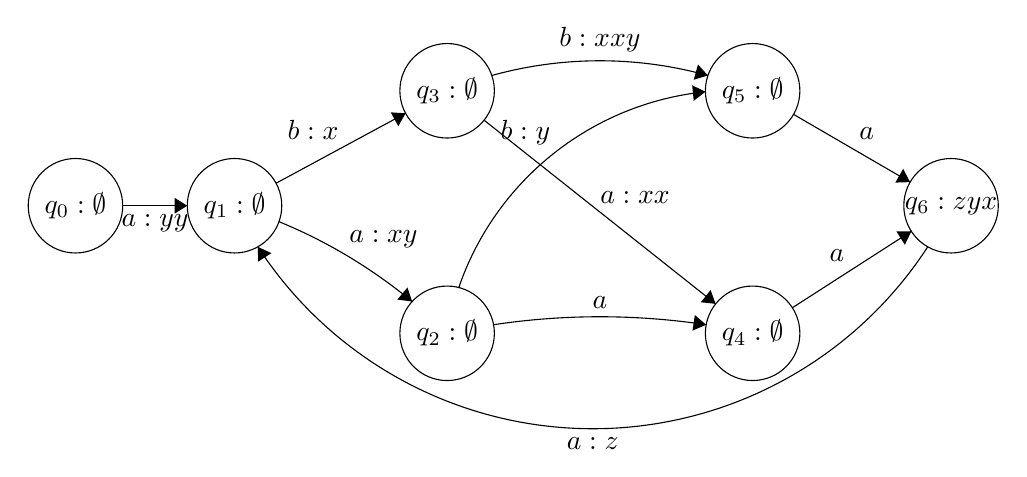
\begin{tikzpicture}[scale=0.2]
	\tikzstyle{every node}+=[inner sep=0pt]
	\draw [black] (26.8,-19.8) circle (3);
	\draw (26.8,-19.8) node {$q_2:\emptyset$};
	\draw [black] (46.2,-19.8) circle (3);
	\draw (46.2,-19.8) node {$q_4:\emptyset$};
	\draw [black] (13.3,-11.7) circle (3);
	\draw (13.3,-11.7) node {$q_1:\emptyset$};
	\draw [black] (26.8,-4.4) circle (3);
	\draw (26.8,-4.4) node {$q_3:\emptyset$};
	\draw [black] (46.2,-4.4) circle (3);
	\draw (46.2,-4.4) node {$q_5:\emptyset$};
	\draw [black] (58.8,-11.7) circle (3);
	\draw (58.8,-11.7) node {$q_6:zyx$};
	\draw [black] (3.2,-11.7) circle (3);
	\draw (3.2,-11.7) node {$q_0:\emptyset$};
	\draw [black] (29.75,-19.255) arc (98.57094:81.42906:45.295);
	\fill [black] (43.25,-19.26) -- (42.53,-18.64) -- (42.38,-19.63);
	\draw (36.5,-18.25) node [above] {$a$};
	\draw [black] (15.94,-10.27) -- (24.16,-5.83);
	\fill [black] (24.16,-5.83) -- (23.22,-5.77) -- (23.7,-6.65);
	\draw (18.28,-7.55) node [above] {$b:x$};
	\draw [black] (16.123,-12.711) arc (67.67284:50.39965:32.833);
	\fill [black] (24.58,-17.78) -- (24.28,-16.89) -- (23.64,-17.66);
	\draw (22.76,-14.43) node [above] {$a:xy$};
	\draw [black] (29.637,-3.43) arc (105.52925:74.47075:25.634);
	\fill [black] (43.36,-3.43) -- (42.73,-2.73) -- (42.46,-3.7);
	\draw (36.5,-1.99) node [above] {$b:xxy$};
	\draw [black] (27.541,-16.896) arc (161.04627:95.83983:18.557);
	\fill [black] (43.2,-4.46) -- (42.36,-4.05) -- (42.46,-5.04);
	\draw (31.77,-7.89) node [above] {$b:y$};
	\draw [black] (29.15,-6.27) -- (43.85,-17.93);
	\fill [black] (43.85,-17.93) -- (43.53,-17.05) -- (42.91,-17.83);
	\draw (38.73,-11.6) node [above] {$a:xx$};
	\draw [black] (48.8,-5.9) -- (56.2,-10.2);
	\fill [black] (56.2,-10.2) -- (55.76,-9.36) -- (55.26,-10.23);
	\draw (53.44,-7.55) node [above] {$a$};
	\draw [black] (48.72,-18.18) -- (56.28,-13.32);
	\fill [black] (56.28,-13.32) -- (55.33,-13.33) -- (55.87,-14.18);
	\draw (51.56,-15.25) node [above] {$a$};
	\draw [black] (6.2,-11.7) -- (10.3,-11.7);
	\fill [black] (10.3,-11.7) -- (9.5,-11.2) -- (9.5,-12.2);
	\draw (8.25,-12.2) node [below] {$a:yy$};
	\draw [black] (57.32,-14.307) arc (-32.97917:-147.02083:25.355);
	\fill [black] (14.78,-14.31) -- (14.8,-15.25) -- (15.64,-14.71);
	\draw (36.05,-26.36) node [below] {$a:z$};
	\end{tikzpicture}
\end{center}

As we can see, if we can jump from state $q_i$ directly to state $q_j$ after reading one single input symbol $\sigma$, then we put transition from $q_i$ to $q_j$ with input label $\sigma$. All the output strings that we pass on our way are put as transition output.

It's possible to specify transition weights in the exact same manner as we do for outputs. We can extend the syntax as follows

\begin{grammar}
	
	<regex> ::= <regex> <regex> // concatenation
	\alt <regex> `|' <regex> //union
	\alt <regex> <weight> //weight after regex
	\alt  <weight> <regex> //weight before regex
	\alt <regex> `*'              //Kleene closure
	\alt `:' <atomic> //output string
	\alt <atomic> //input string
	
\end{grammar}

This syntax is ambiguous. Any weight between two symbols $\sigma_1 w \sigma_2$ could be seen as "before" $\sigma_2$ or "after" $\sigma_1$. This should not be a problem, because no matter how we parse it, the end result is equivalent. (In fact, the real grammar implemented by Solomonoff is the unambiguous version of the syntax above and can be found in \texttt{SolomonoffGrammar.g4}).
Whenever we have several consecutive weights appearing one after the other $\sigma_1 w_1 w_2 \sigma_2$, we  "concatenate" them together. We can do that because $W$ is a monoid that acts on $E$ and this action is associate. Recall that during concatenation, we need to perform left action $pe$ for every final edge $p\in P$ of $lhs$ and initial edge $e\in E$ of $rhs$. If we put weight between them $pwe$, then due to associativity, the order of operations doesn't matter $(pw)e=p(we)$. 

Solomonoff uses lexicographic arctic semiring \cite{MendozaDrosik2020MultitapeAA}. All the implementations specific to this one particular semiring can be found in the class
\texttt{LexUnicodeSpecification}. In the future we might add more semirings, each of which implements \texttt{Specification} in it's own way.  

Lexicographic weights have many useful properties. One of them is that, the previous "history" of weights can be erased and only the weight of last transition is decisive whenever non-deterministic ambiguities arise. This is because the semiring is free. The total weight accumulated when traversing consecutive transitions is obtained by concatenating the weights from each transition. More on this can be found in our other papers \cite{MendozaDrosik2020MultitapeAA}. What's important here, is that each transition must be weighted with exactly one single symbol. For instance if $W=\{w_1,w_2,w_3\}$, then one transition could only be weighted with either $w_1$, $w_2$, $w_3$, but concatenated weights like $w_1w_1$, $w_3w_1$ or $\epsilon$ are not allowed. This poses a problem, because it's possible to create expressions like \texttt{'a' $w_1$ 'b'* $w_2$ 'c'}. Because the subexpression \texttt{'b'*} accepts the empty word, it's possible to jump from \texttt{'a'} straight to \texttt{'c'} and the total of weights on our way would be $w_1 w_2$. That's why the monoid defined in
\begin{lstlisting}[language=java]
W multiplyWeights(W lhs, W rhs)
\end{lstlisting}
must be a different operation, than the multiplication of lexicographic semiring. It's important not to confuse the two!
In Solomonoff $W$ is defined to be $\mathbb{Z}$ (64-bit integers more precisely) and the monoid on $W$ is defined by integer addition. The lexicographic semiring on $W$ is a different entity. Hence the regular expression like \texttt{'a' 3 'b'* -4 'c'} will result in transition from \texttt{'a'} to \texttt{'c'} with weight $3+(-4)=-1$. Defining monoid $W$ as $(\mathbb{Z},+)$ has its own benefits. It allows for automatically inferring weights for any regular expression.


\section{Variables}

The original version\cite{GLUSHKOV} of Glushkov's construction works by first linearizing the regular expression and then recursively finding all 2-factors. It's difficult to apply such approach for regular expressions extended with variables, because the linearization phase works globally and cannot be executed on several subexpressions in parallel. Our version based on singly-linked graphs addresses this problem. Linearization is no longer necessary and it's possible to independently build graphs for many subexpressions, even in parallel. This allows us to extend the compiler with support for variables. The only limitation is that no cyclic dependencies are allowed. For instance consider this equation, where the variable is marked bold
\[
	\boldsymbol{v_1} = a|b\boldsymbol{v_1}  
\]
It might be possible to use Arden's theorem to expand the cyclic dependency using Kleene closures
\[
	\boldsymbol{v_1} = a|b(a|b(a|b(...)))=b^*a
\]
Unfortunately, Arden's theorem can only be applied  in very specific cases and it's easy to devise a cyclic dependency that is not regular. For instance this
\[
	\boldsymbol{v_1} = a\boldsymbol{v_1}a|\epsilon 
\]
is equivalent to
\[
\boldsymbol{v_1} = a^na^n \mbox{ for } n=0,1,2,...
\]
which is a classical example context-free language. To address this issue, Solomonoff only allows for using previously defined variables. No forward declarations or self-references are permitted and no circular dependencies can arise. 
Variables are compiled in the order of definition each one producing some singly-linked graph. Whenever the variables is referenced from some other, the previously evaluated graph is copied in place of the variable and then compilation proceeds as usual. Attention must be paid to always make a deep clone of the entire graph. If we reused graphs without cloning, the compilation could become corrupt. For instance in a regular expression like this
\[
\boldsymbol{v_2} = \boldsymbol{v_1}a|\boldsymbol{v_1}b
\]
the graph stored under the first variable $\boldsymbol{v_1}$ would participate in concatenation twice. Once it is concatenated with $a$ and once with $b$. This would violate the specification of
\begin{lstlisting}[language=java]
/**consumes lhs and rhs*/
G concat(G lhs, G rhs){...}
\end{lstlisting}
which tells us that both parameters are consumed and should not be reused. Solomonoff could in theory clone the variables every single time but there are cases in which the copies could be avoided. For instance user might want to refactor some large expression and for better readability put some subexpressions in their own auxiliary variables. Such variables would only exist for the sole purpose of being used in that one place and there would be no problem to use their graphs directly without cloning. Another more important example would be the case when some large graph on millions of states has been automatically generated from a large dictionary-like dataset. The user might want to perform some simple post-processing, like wrapping the dictionary in Kleene closure or adding some prefix. Cloning the entire graph only to perform a few simple operations could be prohibitively expensive. For this reason Solomonoff implements support for linear logic.

The class \texttt{ParseSpecs} contains all functions necessary for handling variables, types and the general dynamically changing state of compilation. The state is composed of all currently defined variables. The way to interact with it is by invoking the following functions
\begin{lstlisting}[language=java]
Var consumeVariable(String varId)
Var introduceVariable(String name, Pos pos, G graph, 
    boolean alwaysCopy)
Var copyVariable(String var)
Var borrowVariable(String var)
\end{lstlisting}
Whenever a variable is defined, the \texttt{introduceVariable} is called. Then the graph stored under the specific can be referenced from other variables. There are two ways a reference can be used, either with or without exponential operator the \texttt{!!}. By default the \texttt{consumeVariable} is invoked and as a result, the variable is removed from current compilation state after being used. If a reference is done via exponential operator \texttt{!!}, then  \texttt{copyVariable} is invoked instead and the variable remains in the compilation state after being used. For instance in \texttt{v2 = !!v1 'a' | v1 'b'} the first reference uses exponential, so \texttt{v1} is copied and concatenated with \texttt{'a'}. Then the second reference doesn't use \texttt{!!}, so \texttt{v1} is used without copying. Its original graph is concatenated with \texttt{'b'}  and the variable is removed from current compilation state. 
Another interesting example is \texttt{v1 = v1 'b'}. It might look like a circular dependency but in fact it is not. In the presence of linear logic it should should be understood as taking the graph from \texttt{v1}, removing \texttt{v1} from compilation state, concatenating the graph with \texttt{'b'} and then introducing a brand new variable but under the same name \texttt{v1}. One way to think about it is that we reassigned \texttt{v1}. In this sense linear logic can be used to model mutations. This should not be confused with mutations that often occur most other programming languages. Things like \texttt{v1 = !!v1 'b'} are not allowed and would result in error. Compiler would see it as an attempt to define \texttt{v1} twice.

\section{External functions}

As it was shown above, by reinventing Glushkov's construction in terms of graphs, we were able to compile different subexpressions independently, store them under variables and reuse as many times as we want. The next idea that naturally comes to mind is to manipulate such graphs using some external procedures. This way we can introduce operations that  would otherwise never be possible in plain Glushkov's construction.
The class \texttt{ParseSpecs} contains two methods for calling external procedures
\begin{lstlisting}[language=java]
G externalFunction(Pos pos, String functionName, 
    List<Pair<O, O>> args);
G externalOperation(Pos pos, String functionName, 
    List<G> args);
\end{lstlisting}
The difference between the two is subtle and in the future they will likely be unified into one common method. Users are free to add their own external functions via
\begin{lstlisting}[language=java]
ExternalFunction<G> registerExternalFunction(
    String name, ExternalFunction<G> f)
ExternalOperation<G> registerExternalOperation(
    String name, ExternalOperation<G> f)
\end{lstlisting}
found in \texttt{LexUnicodeSpecification}.

A galore of external utility functions has been implemented throughout the library. The more generic implementations are kept in \texttt{Specification}, while other procedures that are specific to lexicographic semiring are placed in \texttt{LexUnicodeSpecification}. We present a brief summary of the most important procedures.

The most important building block and base for most other procedures is the \texttt{collect} function, which explores the reachable structure of graph in depth-first order.
\begin{lstlisting}[language=java]
S collect(G graph, N startpoint, S set,
Function<N, Object> shouldContinuePerState,
BiFunction<N, E, Object> shouldContinuePerEdge)
\end{lstlisting}
It is highly customisable and can be used both for collecting all vertices and searching the graph for a vertex or edge satisfying specific property. If the user is not interested in exploring entire graph, it's possible to terminate early by returning non-null value from either \texttt{shouldContinuePerState} or \texttt{shouldContinuePerEdge}. 

Another highly ubiquitous function is \texttt{collectProduct}. It works similarly to \texttt{collect}, but it traverses two automata simultaneously.  This strictly implements the cross product of automata. The starting point is the pair of unique initial states of the respective automata. Then it iteratively find successive  pair of states that can be reachable by traversing transitions over the same input. To visualise it, one might imagine that we choose some input string and then see what states can be reached in both automata. We collect all pairs of states that can be simultaneously reached when reading some input string.
This procedure heavily depends on other \texttt{zipTransitionRanges}. As we already presented above, a way to build an efficient lookup table $c_1<c_2<...<c_n$ for any set of outgoing transitions. It is
then possible to efficiently zip such table with another one, say $d_1<d_2<...<d_m$  and obtain cross product of transition tables that may look more or less like
$c_1<c_2<d_1<c_3<d_2<d_3<...<c_n<...<d_m$. This makes the \texttt{collectProduct} work very efficiently even for alphabets consisting of millions of symbols.

Those functions are the basis for other more specialised procedures. The advance-and-delay \cite{Marie-Pierre} is implemented in \texttt{advanceAndDelay} as a particular case of \texttt{collectProduct}. Then equivalence test \texttt{areEquivalent} for deterministic transducers is implemented as a special case of  \texttt{advanceAndDelay}. 

Testing if language of one automaton is a subset of another is implemented in \texttt{isSubset}, which also is a special case of 
\texttt{collectProduct}.

In case of transducers it's possible to define an operation similar to \texttt{collectProduct} but instead of zipping two automata's input, it zips the output of first transducer with output of second one. This is implemented in \texttt{collectOutputProductDeterministic}. This function assumes that the first transducer is deterministic. (Otherwise the procedure would become exponential.) 

It's possible to check whether the output language of one transducer is a subset of the input of another. This is done in \texttt{isOutputSubset} and the implementation is a special case of \texttt{collectOutputProductDeterministic}. 

Language difference is implemented in \texttt{subtract} and it's also based on \texttt{collectProduct}.

There are several heavy-weight functions that are not a special case of anything else. The
\texttt{inverse}  swaps inputs of transducer with its own outputs. As a result the input language becomes the output and vice versa. It requires the transducer to be bijective or otherwise, the inversion would not be functional. A more general inversion, which works with non-bijective transducers is experimentally implemented at syntactic level and manipulates the regular expressions rather than automata. More precisely, in order to invert an expression it's enough to turn all input strings into output strings and vice-versa. For instance the inverse of \texttt{('a':'b')*:'c'} becomes \texttt{(:'a' 'b')* 'c'}. 

There is a procedure for \texttt{powerset} construction. In case of transducer, the resulting automaton is stripped of all its outputs, because the powerset operation is only defined for finite state automata and not transducers. It's possible to extend the powerset construction to a special version for transducers but there was no need to implement it in Solomonoff so far. 

There is a \texttt{compose} procedure, taking two transducers and producing a third one that simulates function composition determined by of the two.

Solomonoff has a \texttt{trim} procedure, which removes all dead-end states. Trim automata by definition have no unreachable and no unobservable (dead-end) states. Singly linked graphs guarantee that all states are automaton only consist of reachable vertices. Glushkov's construction guarantees that all states are observable. Therefore the \texttt{trim} procedure is generally not needed. There are only a few external operations that may introduce unobservable states and then the trimming might need to be performed explicitly.

There is a way to generate \texttt{randomDeterministic} automata. \texttt{generate} allows for randomly sampling some inputs/outputs or even enumerating entire languages of transducers.

All of the above functions are highly customizable. They often take higher order functions as parameters, which allows for specifying custom behaviour on various events. 

One could notice that some of the functions work with \texttt{RangedGraph<V, In, E, P>} instead of \texttt{G}. The \texttt{RangedGraph} implements the efficient transition lookup table. Procedures that make have use of symbol lookups tend to use \texttt{RangedGraph} over plain \texttt{G}.  


Many of the functions are exposed for use directly in regular expressions via the interface of external operations. Those include \\
\texttt{compose[arg1,arg2,arg3...]}, \\
\texttt{subtract[lhs,rhs]}, \\
\texttt{random!()} \\
\texttt{inverse[arg]} and several others.



\bibliographystyle{BibTeXtran}   % (uses file "BibTeXtran.bst")
\bibliography{BibTeXrefs}    







\end{document}
